\section{Use cases}
	In this section we present the use cases for our application.
	\begin{enumerate}
		\item Registration: The first time a user use this application he will be asked to registr himself, providing a username and a password, and specifying which type of user he/she is (customer or ristorateur).
		After this, the User can Login and start to use the application.
		\item Login/Logout: A User (customer or ristorateur), will provide his credentials, the application will check if he/she is registered (present in the DB) and then will grant or deny the access, depending on the result of the check.
		\item List Restauraunts: The list of all available restauraunts, with description, genre, price, and number of seats available will be provided to the Customer, he/she will choose among these where to make a reservation.
		\item List Reservations: The list of all the reservation made from a Customer will be provided to him/her, in order to check the date and hour, or the address of the restauraunt.
		\item Add/Modify Restauraunt: A Restaurateur will be able to Add/Modify a restauraunt, obviously only the owner of a restauraunt can modify it.
		\item List Restoauraunt Reservation: A restaurateur can use this in order to know how many reservation have been taken in his restauraunts, a list of reservations, ordered by restauraunt, will be provided to him by the application, only the reservations in the future will be shown.
	\end{enumerate}

\begin{figure}
  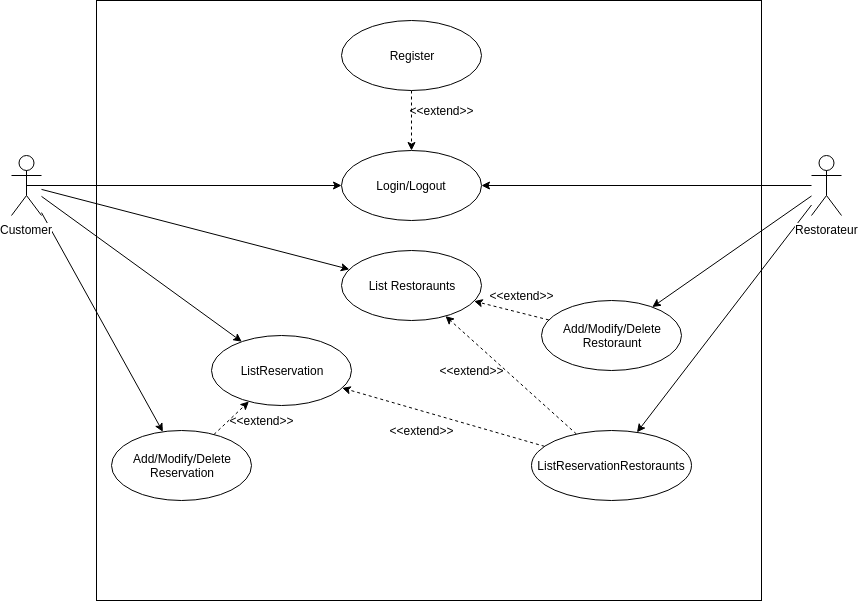
\includegraphics[width=\linewidth]{USE_CASE.png}
  \caption{Use cases diagram.}
  \label{figureUSE_CASE}
\end{figure}

\pagebreak